\documentclass{article}

\usepackage{arxiv}

\usepackage[utf8]{inputenc} % allow utf-8 input
\usepackage[T1]{fontenc}    % use 8-bit T1 fonts
\usepackage{hyperref}       % hyperlinks
\usepackage{url}            % simple URL typesetting
\usepackage{booktabs}       % professional-quality tables
\usepackage{amsfonts}       % blackboard math symbols
\usepackage{nicefrac}       % compact symbols for 1/2, etc.
\usepackage{microtype}      % microtypography
\usepackage{lipsum}		% Can be removed after putting your text content
\usepackage{amssymb,amsmath}
\usepackage{listings}
\usepackage{graphicx}
\usepackage{subfig}
\usepackage{apacite}

\title{Contact-tracing strategies for SARS-CoV-2 eradication
\textbf{**** DRAFT ****}
}

%\date{September 9, 1985}	% Here you can change the date presented in the paper title
%\date{} 					% Or removing it

\author{
  Daniel Tang\\
  Leeds Institute for Data Analytics\thanks{This project has received funding from the European Research Council (ERC) under the European Union’s Horizon 2020 research and innovation programme (grant agreement No. 757455)}\\
  University of Leeds\\
  Leeds, UK\\
  \texttt{D.Tang@leeds.ac.uk} \\
  %% examples of more authors
  %% \AND
  %% Coauthor \\
  %% Affiliation \\
  %% Address \\
}


\begin{document}
\maketitle

\begin{abstract}
As of $5^{rd}$ April a large proportion of the global population are living under social distancing measures in order to control the spread of COVID-19. If these measures are successful, in a few weeks, prevalence will again be low in certain parts of the world. However, it is not clear what the best policy will be at that point. This paper investigates the feasibility of using contact tracing along with a combination of other measures in order to ease the social distancing measures while preventing a resurgence of the disease. We find that manual contact tracing alone is unlikely to achieve the speed or accuracy needed to contain the disease, and so suggest a technological solution based on tracing via mobile phone app. The proposed solution maintains user's privacy and conforms to European data protection laws.
\textbf{**** This is a live document and is subject to change ****}

\end{abstract}

% keywords can be removed
\keywords{COVID-19, SARS-CoV-2}

\section{Introduction}

Many countries in the world are now committed to a surge in incidence of COVID-19 and are practising social distancing in order to suppress its spread. If successful, these countries will soon be in a situation where prevalence is reducing. Once this is achieved there are a number of strategies:
\begin{itemize}

\item lift the social distancing measures and allow a second (and subsequent) waves until herd immunity is achieved\cite{ferguson2020impact}.

\item maintain low levels until a vaccine is available

\item eradicate the virus locally and impose strict border controls and containment strategies until the virus is contained globally
\end{itemize}

Here we investigate the feasibility of the third option by slowly lifting social distancing measures while maintaining self isolation of symptomatic individuals and implementing an extensive testing and contact-tracing capability.

\section{Description of the Model}

The model we use is based on the stochastic branching model described in \cite{hellewellfeasibility} but implemented as an agent-based, discrete event simulation. This allows us to implement more complex containment strategies with less effort. It also allows us to correctly capture the tracing of infected agents via a previously untraced mutual infector, which is not properly captured in a stochastic branching model. In the presence of many asymptomatic carriers, and very fast and accurate tracing, this is expected to be important. It also allows us to capture the workload on a central testing facility and the feedback of delays as workload increases.\footnote{Although a discrete-event simulation takes longer to execute than a branching model, execution time is not a bottleneck so it is worthwhile in order to capture these dynamics.} 

The model consists of infected agents, each of which belongs to a household and a workplace/school. Once infected, an agent goes though an incubation period with duration drawn from a Weibull distribution with shape parameter $2.322737$ and scale parameter $6.492272$\cite{backer2020incubation}. The transmission generation interval (i.e. time from exposure to transmission) is drawn from a skew normal distribution with location parameter equal to the clinical onset time (i.e. end of the incubation period), scale parameter of 2.0 and skew parameter of 1.95\cite{hellewellfeasibility}. This results in 15\% of infections occurring before clinical onset\cite{hellewellfeasibility}. In order to avoid unrealistically early transmissions, the generation interval was bounded to a minimum of 1 day. At creation, $17.9\%$ of agents are deemed to be asymptomatic\cite{:/content/10.2807/1560-7917.ES.2020.25.10.2000180}\footnote{[TODO: Age weight this figure]}. Asymptomatic carriers are assumed to be $\frac{2}{3}$ as infectious as symptomatic carriers\cite{ferguson2020impact}. The number of susceptible agents that an infected agent will infect if not isolated is drawn from a negative binomial distribution with overdispersion parameter $10.0$\cite{zhuang2020preliminary}\cite{riou2020pattern} and mean of $\frac{3R_0}{3 - \rho}$ for symptomatic agents and $\frac{2R_0}{3 - \rho}$ for asymptomatic agents where $\rho=0.179$ is the probability of being asymptomatic and $R_0$ is the basic reproductive number. At each transmission event a new infected agent is created, unless the agent is isolated, in which case the event has no effect.

Each transmission event occurs either in the household, at the workplace/school or in the community. This allows us to capture the differences in ease and speed of contact tracing in these three cases, as well as capturing the effect of closer and more frequent contact with household members compared to workplace and community. Distinguishing household contacts also allows us to simulate the effect of household-wide self-isolation policies such as those implemented in the UK. Finally, it allows us to capture any immunity in the population built up during a first wave of infections. After a first wave of infection we would expect there to be a correlation in immunity between members of the same household since during the peak, under ``stay at home'' rules, if one member of a household contracts the disease it is likely that all other members will also contract it, so we end up with immune and susceptible households. This means that only members of susceptible households can become infected during the contact-tracing stage. The relative probability of transmission in the household was 3 times greater in the household than in the other locations. This calibrated in order to obtain equal aggregate numbers of transmission events in each location under no intervention\cite{ferguson2020impact}. The distribution of number of members in a household was calibrated against\cite{smithHouseholds}. A transmission event to an immune agent does not cause infection. Immunity is only applied to school/workplace and community transmissions for the reasons outlined above.

The source code of the model is available at \href{https://github.com/danftang/Covid19}{https://github.com/danftang/Covid19}

\section{Policy Scenarios}

Various policy scenarios were simulated to find the probability that an initial population of 100 infected agents could be eradicated. Eradication was deemed to have been achieved if the cumulative number of cases remained below 5000 and there was no untraced infected population at 15 weeks into the simulation. It was assumed that $5\%$ of the population was immune. The probability of eradication was estimated by performing a monte-carlo run of 300 simulations and counting the proportion that achieved eradication.

If not otherwise stated the following default values are used in the scenarios: $15\%$ pre-symptomatic transmission, $R0 = 3.5$, $18\%$ of infected are asymptomatic carriers, $5\%$ of the population are immune and 75\% of people comply with policy. Swab tests take 24 hours to process and come back positive if the agent's infectiousness is above $2\%$ per day, this excludes positive results during the latent phase.

\subsection{Manual contact tracing with household-wide quarantine}

In this scenario, anyone who becomes symptomatic must immediately self-isolate along with all members of the household. The symptomatic person is tested and if positive close-contacts are traced, quarantined and tested. Further positive results are traced recursively.

In this scenario, the speed and accuracy of the contact tracing is of key importance. Figure \ref{tracingContour} shows the probability of containment for a range of values of the time taken to trace a contact (i.e. perform a test on a suspected case, get results and trace the contact) and of the proportion of close contacts that are traced. This figure is based on the assumption that 75\% of the public comply with the self-isolation policy. As can be seen, the contact tracing would need to be very fast and accurate to have a reasonable chance of containment. For this reason, it seems unlikely that manual contact-tracing, based on interviews with the infected person, will be fast or accurate enough to be effective.

\begin{figure}
\begin{center}
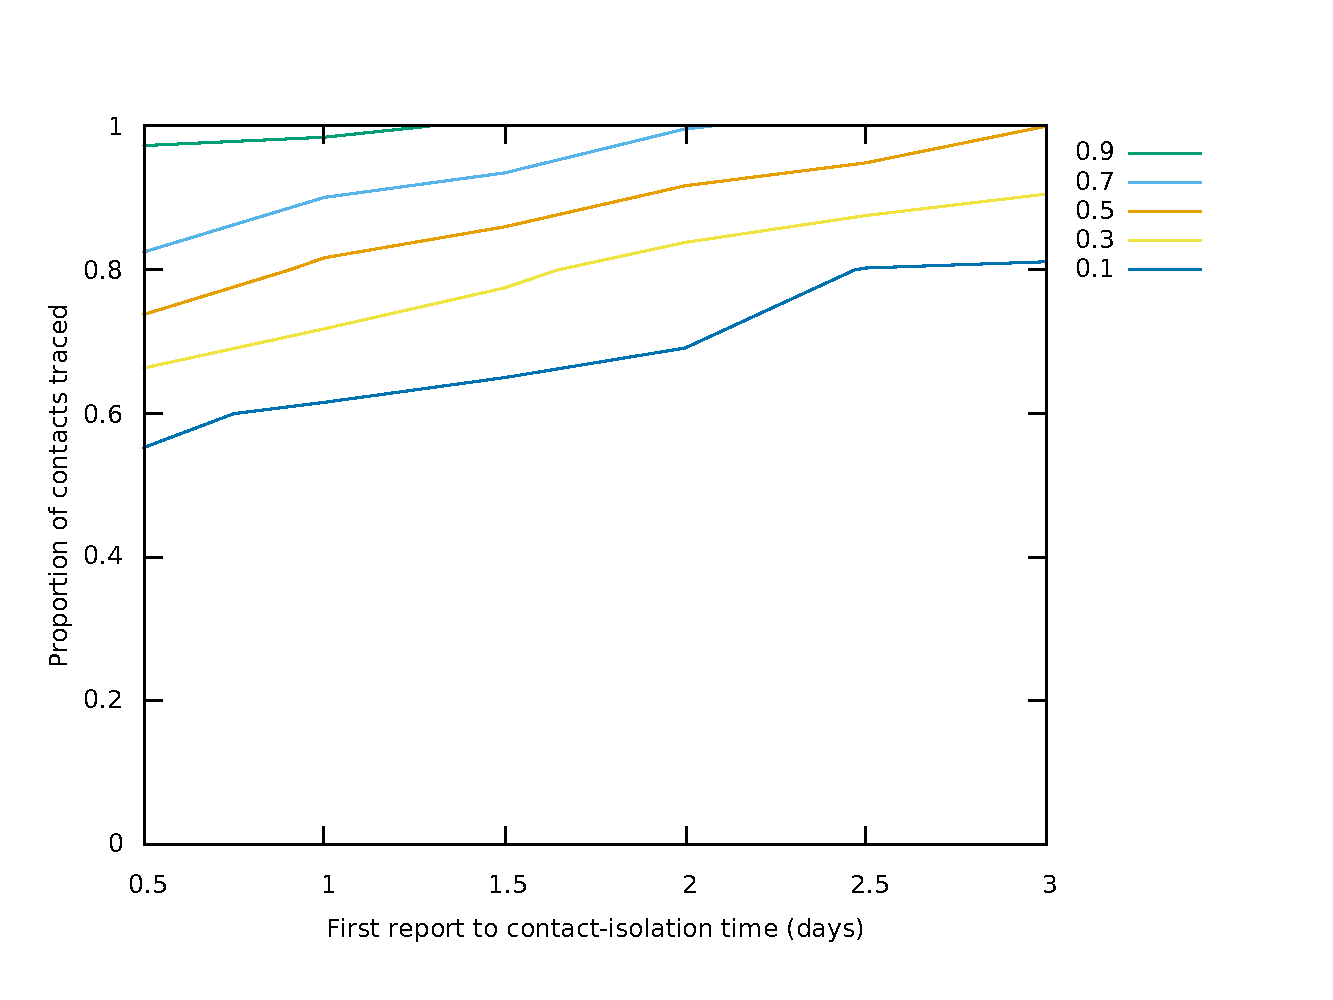
\includegraphics[width = 10cm]{tracingContour.pdf}
\end{center}
\caption{Probability of eradication under self-isolation and contact tracing. Assuming 95\% compliance to self-isolation.}
\label{tracingContour}
\end{figure}

\subsection{Isolation of whole household and work-colleagues}

In this scenario, we have household-wide quarantine as above, but in addition, we assume that companies are (perhaps legally) obliged to report symptomatic employees and have systems in place to record close contacts within the workplace. Under this scenario, we assume that $90\%$ of close contacts within the workplace can be traced and $90\%$ of non-compliant symptomatic cases are reported. The time from first report to isolation of workplace colleagues is taken to be 36 hours, representing the swab test time of 24 hours plus 12 hours delay.

Under this scenario, with the default parameters, all simulations are controlled even without any tracing in the community. With less optimistic values of 30\% pre-symptomatic transmission and 30\% of infections asymptomatic, the probability of control is as shown in figure \ref{householdWorkplace3030}.

\begin{figure}
\begin{center}
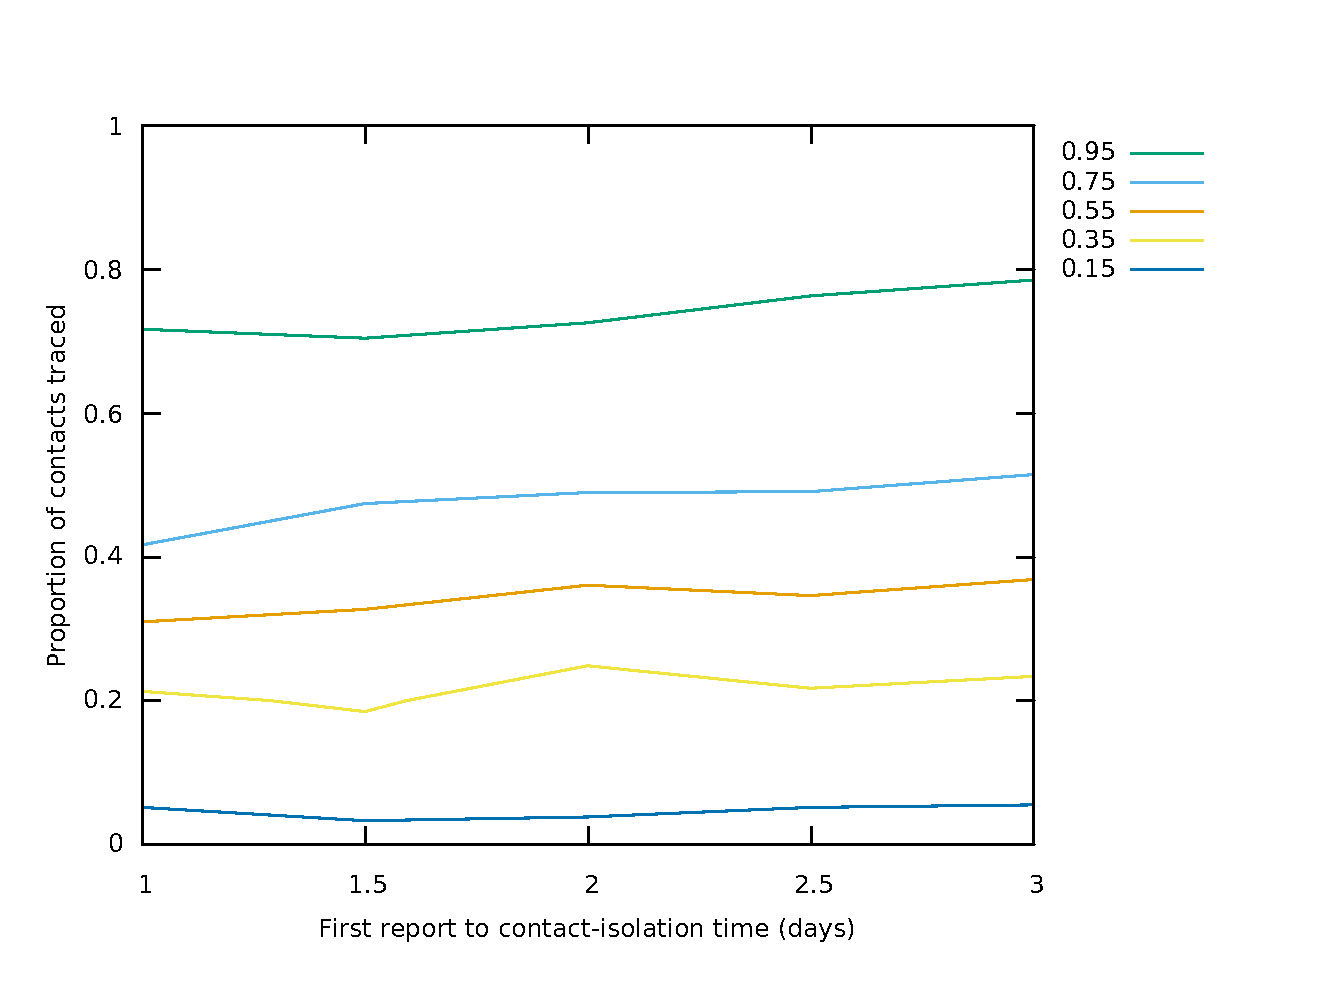
\includegraphics[width = 10cm]{contourWorkplace.pdf}
\end{center}
\caption{Probability of eradication under quarantine of whole household and workplace contacts assuming 90\% enforcement in the workplace, 30\% pre-symptomatic transmission and 30\% of infections asymptomatic.}
\label{householdWorkplace3030}
\end{figure}

In this case, we would need to trace upwards of 80\% of contacts in the community in order to have a >95\% chance of control.

\subsection{Tracing with mobile phone app}

The only practical way of tracing such a high proportion of contacts in the community is by using technology. Efforts to control the virus in China have demonstrated the use of community tracing technology, but implementation in western countries is more challenging because user privacy and data protection must be preserved. However, a privacy-protecting mobile phone app for contact tracing has been proposed\cite{tang2020Mobile}, so in this scenario, we add the use of this mobile app in addition to household self-isolation and workplace enforcement. We assume that the phone app can track 90\% of close contacts between users.

In this scenario we assume compliance is an intrinsic property of the agent. A compliant agent will install the mobile phone app and self-isolate upon becoming symptomatic, whereas a non-compliant agent will do neither. This captures the expected correlation between these things, which is important because it makes it more likely that an infectious person in the community will not be using the mobile phone app, and therefore cannot be traced.\footnote{[Non-compliants are more likely to be immune (what is the size of this effect?)]}

At the default values, all simulations are controlled. However, the probability of control is very sensitive to the proportion of infections that are asymptomatic. Figure \ref{fulltrace25} shows the case where 25\% of infections are asymptomatic and 30\% of transmission is pre-symptomatic. Figure \ref{fulltrace30} shows the same but with 30\% pre-symptomatic transmission.

\begin{figure}
\begin{center}
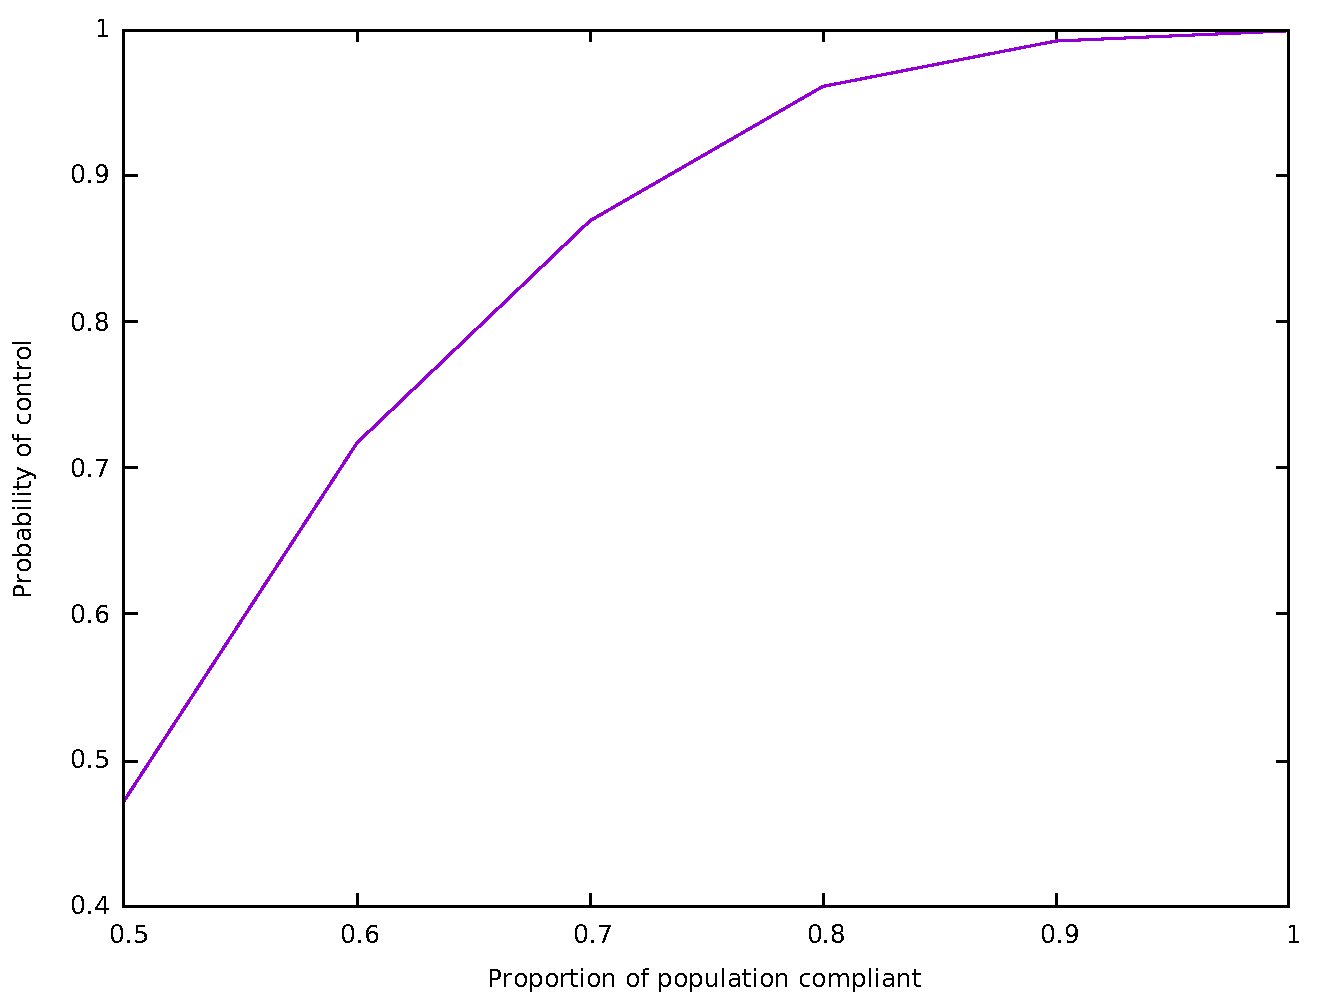
\includegraphics[width = 10cm]{mobileTracing25Subclinical30pre.pdf}
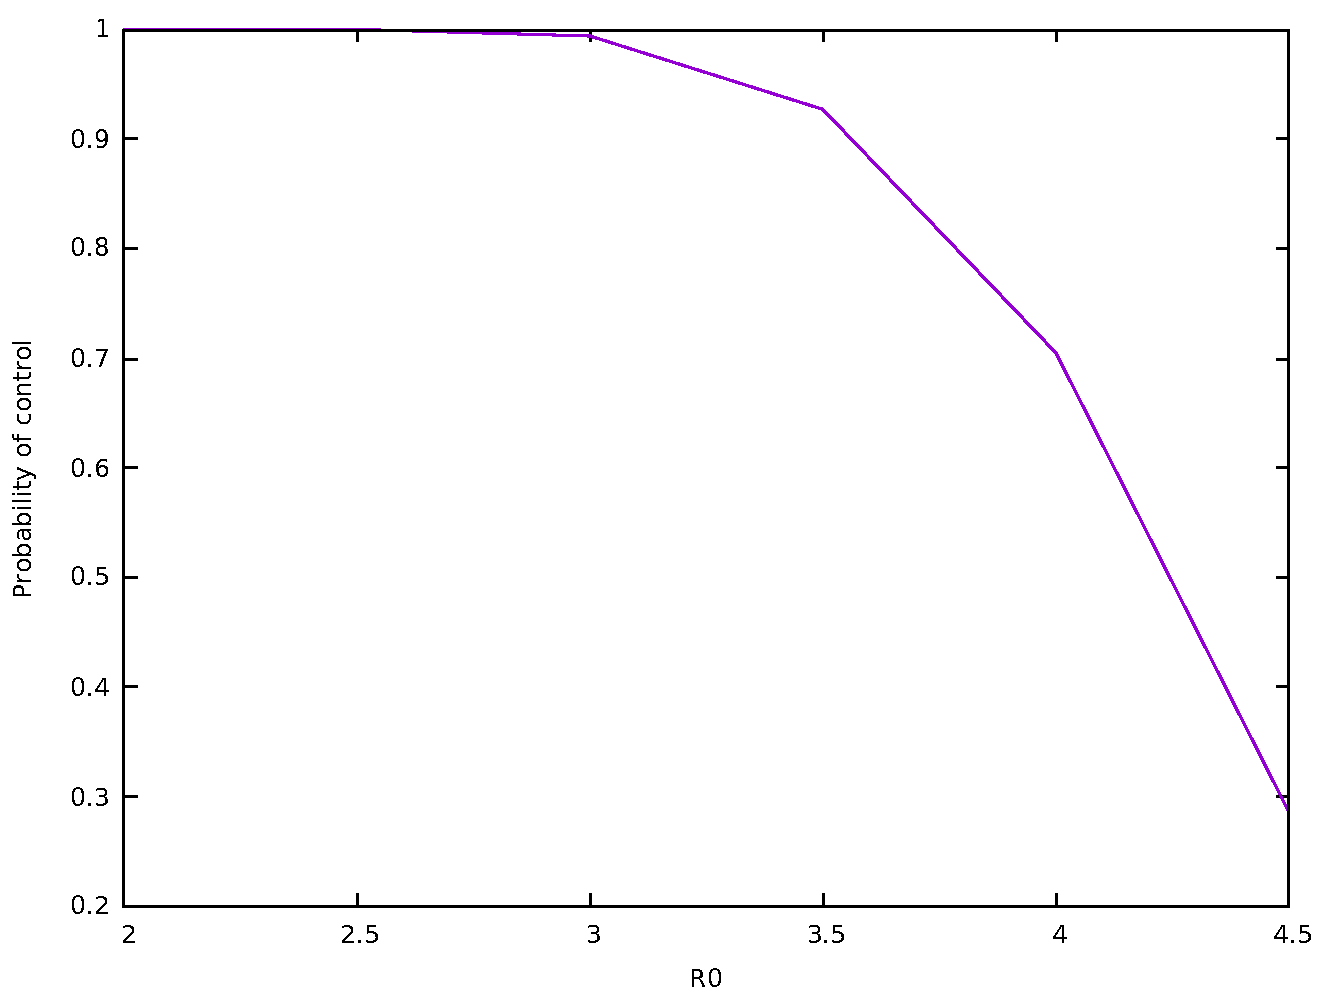
\includegraphics[width = 10cm]{mobileTracing25Subclinical30preR0.pdf}
\end{center}
\caption{Probability of eradication under community tracing assuming 90\% enforcement in the workplace, 30\% pre-symptomatic transmission and 25\% of infections asymptomatic. Averaged over 1000 simulations.}
\label{fulltrace25}
\end{figure}

\begin{figure}
\begin{center}
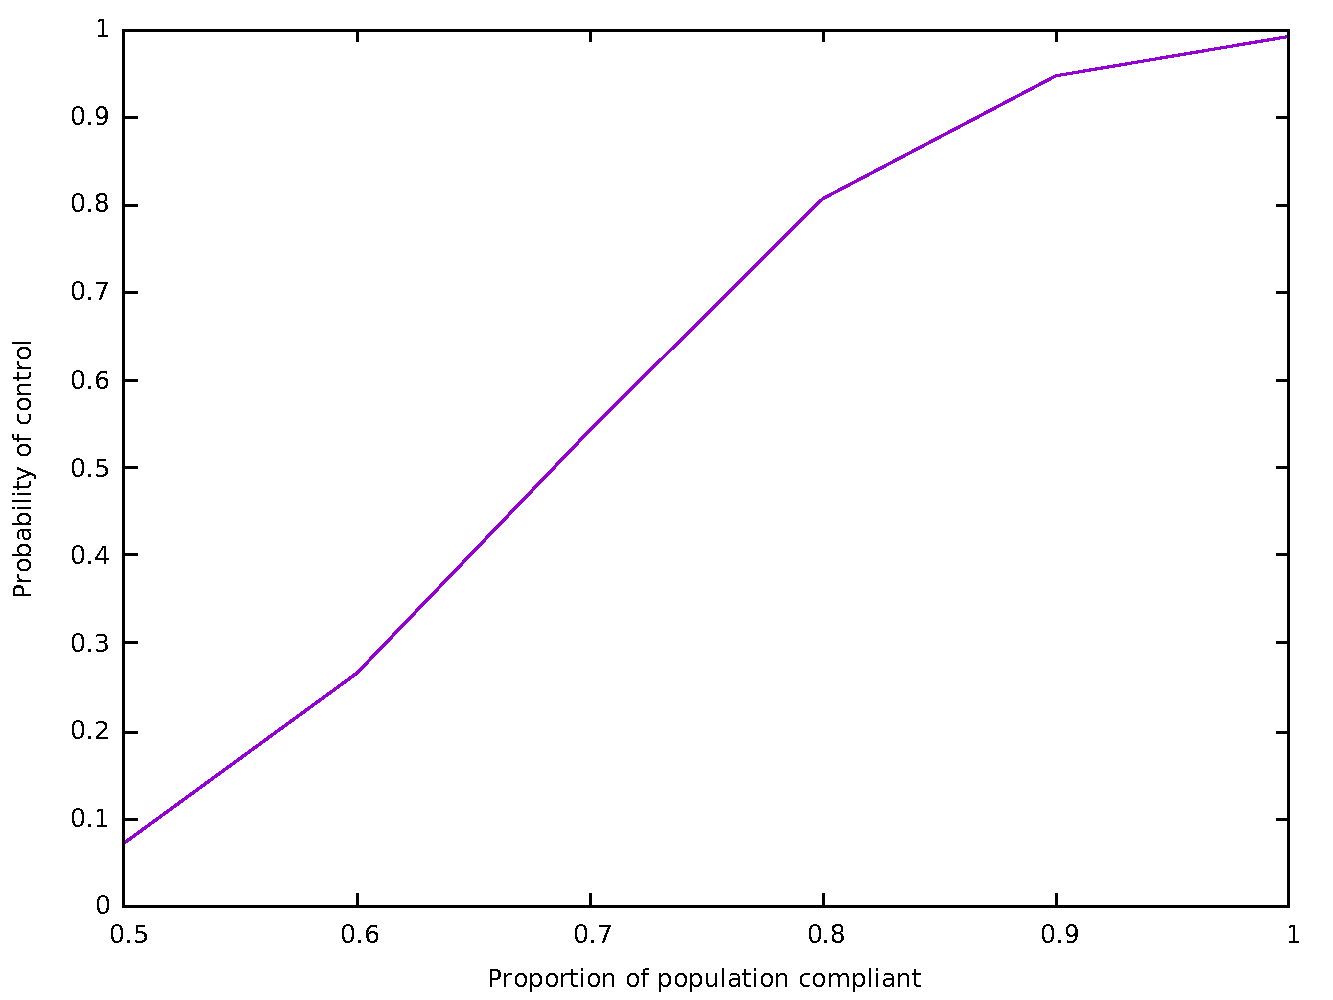
\includegraphics[width = 10cm]{mobileTracing30Subclinical30pre.pdf}
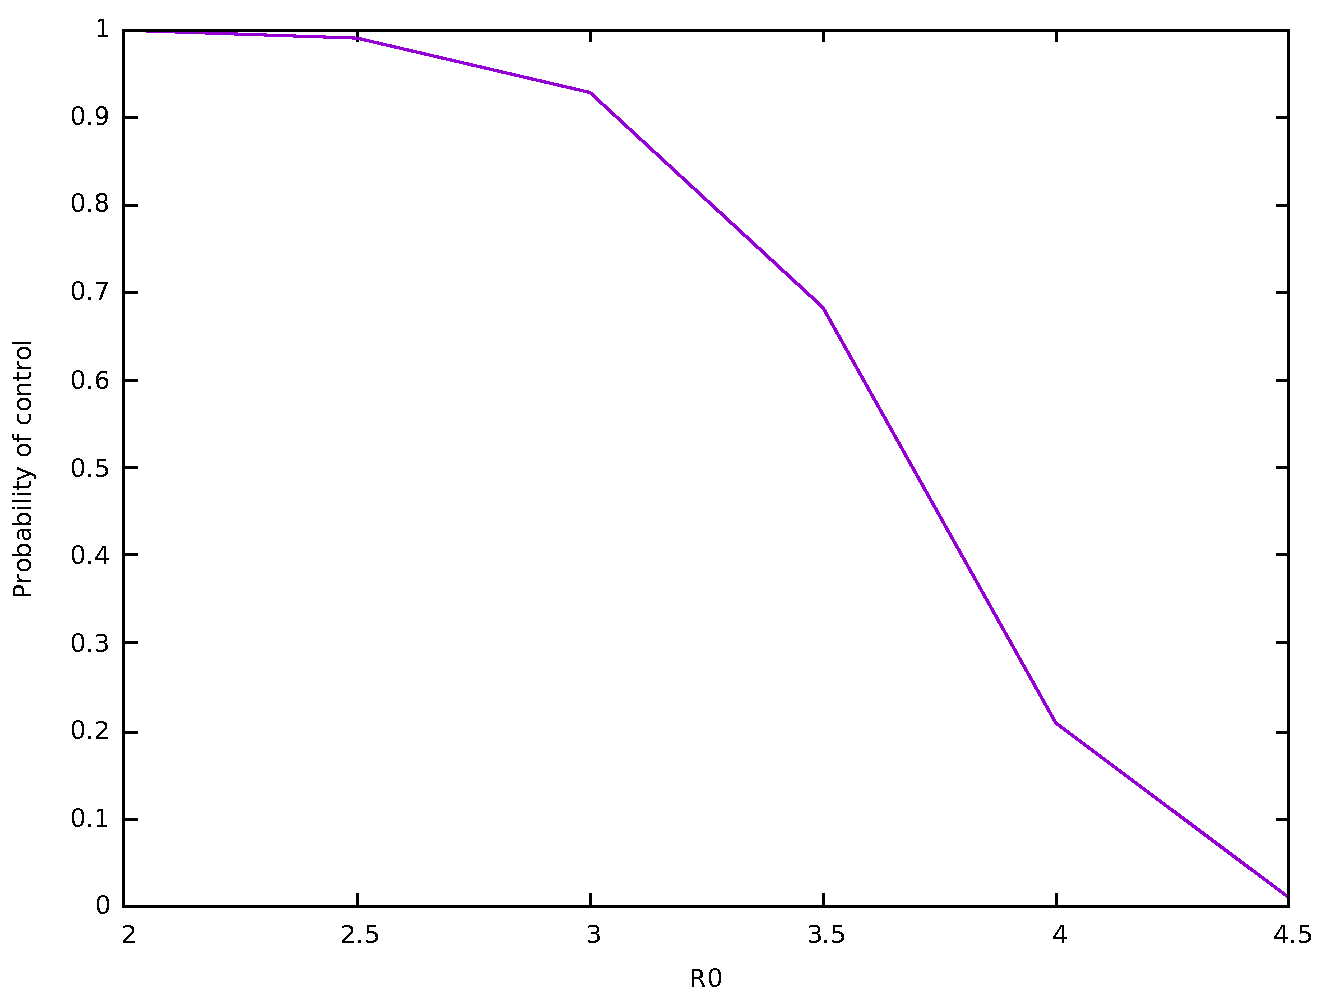
\includegraphics[width = 10cm]{mobileTracing30Subclinical30preR0.pdf}
\end{center}
\caption{Probability of eradication under community tracing with mobile phone assuming 90\% enforcement in the workplace, 30\% pre-symptomatic transmission and 30\% of infections asymptomatic. Averaged over 1000 simulations.}
\label{fulltrace30}
\end{figure}

\section{Discussion}

We have shown that a policy of household-wide isolation along with workplace enforcement and a mobile phone app for community contact tracing has a good chance of controlling outbreaks even under quite pessimistic values of the parameters. However, under these parameters it's success depends on a very high proportion of the population installing the app. A recent survey\cite{abeler2020Support} has shown that public support for an app is high in the UK and that around 74\% of respondents would probably or definitely install a contact-tracing app. In many cases this would be enough, but if, for example, the proportion of asymptomatic carriers turns out to be very high it may be necessary to offer strong incentives to use the app or even make it mandatory.

The range of uncertainty in the parameters is, however, very large and sensitivity to these parameters is high, meaning that, at one extreme, household isolation along with workplace enforcement may be enough to control the disease without any tracing of contacts in the community, while at the other extreme very high uptake of mobile phone tracking would be needed in combination with some continued social distancing.

Under such large uncertainty, the probability of preventing a resurgence of infections can be minimised by adopting a policy of gradual loosening of social distancing measures along with close observation of the data. In this way, the effective $R$ can be gradually increased while constantly using new observations to feed back into the policy by working out if further loosening is possible or more app uptake is necessary.

%\bibliographystyle{unsrtnat}
%\bibliographystyle{apalike} 
\bibliographystyle{apacite}
\bibliography{references}

\end{document}
